% !TeX program = pdflatex
\documentclass[tikz,border=8pt]{standalone}
\usepackage{tikz}
\usetikzlibrary{positioning}
\definecolor{Shade}{HTML}{FED7AA}
\definecolor{FigureBlue}{HTML}{2563EB}
\definecolor{FigureOrange}{HTML}{EA580C}
\definecolor{FigureSlate}{HTML}{475569}
\begin{document}
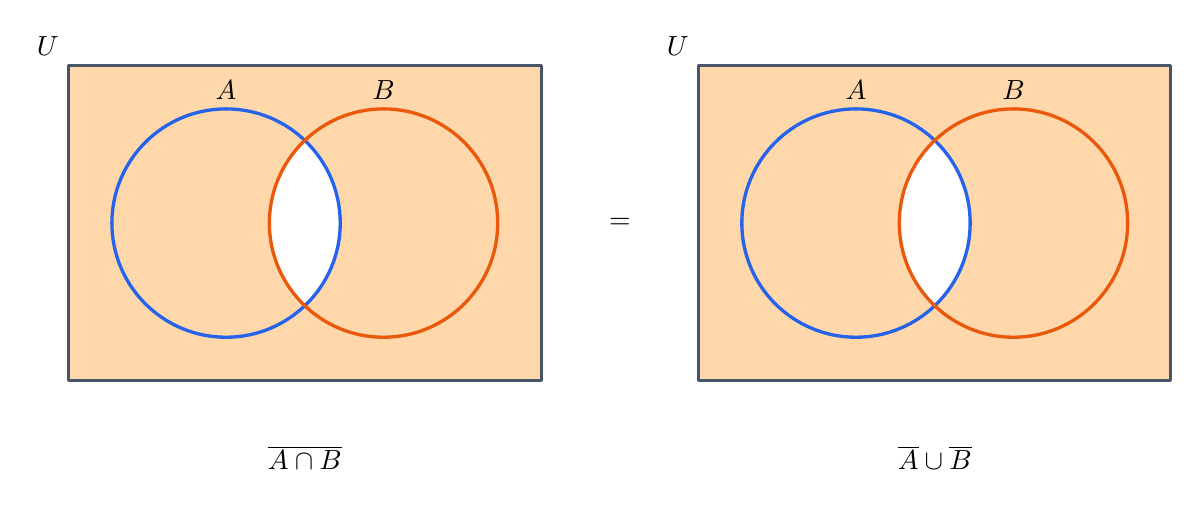
\begin{tikzpicture}[line cap=round,line join=round]
  \begin{scope}
    \fill[Shade] (-3,-2) rectangle (3,2);
    \begin{scope}\clip (-1,0) circle[radius=1.45];\fill[white] (1,0) circle[radius=1.45];\end{scope}
    \draw[FigureSlate,line width=1.1pt] (-3,-2) rectangle (3,2);
    \draw[FigureBlue,line width=1.2pt] (-1,0) circle[radius=1.45];
    \draw[FigureOrange,line width=1.2pt] (1,0) circle[radius=1.45];
    \node[above left] at (-3,2) {$U$};\node[above] at (-1,1.45) {$A$};\node[above] at (1,1.45) {$B$};
    \node[below=7mm] at (0,-2) {$\overline{A\cap B}$};
  \end{scope}
  \node at (4,0) {$=$};
  \begin{scope}[xshift=8cm]
    % Build the union from the two complements; their only common unshaded part is A cap B.
    \path[fill=Shade,even odd rule] (-3,-2) rectangle (3,2) (-1,0) circle[radius=1.45];
    \path[fill=Shade,even odd rule] (-3,-2) rectangle (3,2) (1,0) circle[radius=1.45];
    \draw[FigureSlate,line width=1.1pt] (-3,-2) rectangle (3,2);
    \draw[FigureBlue,line width=1.2pt] (-1,0) circle[radius=1.45];
    \draw[FigureOrange,line width=1.2pt] (1,0) circle[radius=1.45];
    \node[above left] at (-3,2) {$U$};\node[above] at (-1,1.45) {$A$};\node[above] at (1,1.45) {$B$};
    \node[below=7mm] at (0,-2) {$\overline A\cup\overline B$};
  \end{scope}
\end{tikzpicture}
\end{document}
